% !TEX root = wd-full.tex

Having derived constraints on generic models of ultra-heavy DM, we turn towards a concrete example.
In various supersymmetric extensions of the SM, non-topological solitons called Q-balls can be produced in the early universe~\cite{Coleman:1985ki, Kusenko:1997si}.
If these Q-balls were stable, they would comprise a component of the DM today.
For gauge-mediated models with flat scalar potentials, the Q-ball mass and radius are given by
\begin{equation}
\label{eq:Qballprop}
M_Q \sim m_S Q^{3/4}, ~~~ R_Q \sim m_S^{-1} Q^{1/4},
\end{equation}
where $m_S$ is related to the scale of supersymmetry breaking, and $Q$ is the global charge of the Q-ball---in our case, baryon number.
The condition $M_Q/Q < m_p$ ensures that the Q-ball is stable against decay to nucleons.
When a baryonic Q-ball interacts with a nucleon, it induces the dissociation of the nucleon and absorbs its baryonic charge.
During this proton decay-like process, excess energy of order $\Lambda_\text{QCD}$ is released via the emission of 2--3 pions~\cite{Kusenko:1998}.
We assume that for each Q-ball inelastic collision, there is equal probability to produce $\pi^0$ and $\pi^\pm$ under the constraint of charge conservation.
The cross section for this interaction is approximately geometric
\begin{align}
\sigma_Q \sim \pi R_Q^2,
\end{align}
and thus grows with increasing $Q$.
Note that a sufficiently massive Q-ball will become a black hole if $R_Q \lesssim G M_Q$.
In the model described above, this translates into a condition $(M_\text{pl}/m_S)^4 \lesssim Q$.

We now determine the explosiveness of a Q-ball transit.
This process is described by a linear energy transfer
\begin{equation}
\label{eq:QballLET}
\l\frac{dE}{dx}\r_\text{LET} \sim n_\text{ion} \sigma_Q N_\pi \epsilon,
\end{equation}
where the nuclear interaction results in $N_\pi \approx 30$ pions released, each with kinetic energy $\epsilon \approx 500 ~\text{MeV}$.
These pions induce hadronic showers which terminate in low-energy hadrons that rapidly transfer their energy to ions via elastic scatters, as discussed in Section~\ref{sec:smheating}.
The pions have a heating length $X_\text{had} \lesssim \lambda_T$; however, we will see the Q-ball has a finite size $R_Q \gtrsim X_\text{had}$ in the region we are able to constrain.
So, as mentioned in Section~\ref{sec:dmignition}, we take the heating length to be $L_0 \sim R_Q + X_\text{had} \sim R_Q$.
The ignition condition is then given by equations~\eqref{eq:transitexplosion} and~\eqref{eq:QballLET}:
\begin{equation}
 R_Q^2 \gtrsim \frac{1}{n_\text{ion}} \frac{\Eboom}{\lambda_T}
 \; \xmax\left \{ \frac{R_Q}{\lambda_T}, 1\right\}^2
 \l \frac{1}{10~\GeV} \r.
\end{equation}
This implies $\sigma_Q \gtrsim 10^{-12} ~\text{cm}^2$ is sufficient to ignite a $1.25 ~M_{\astrosun}$ WD, which corresponds to a charge $Q \gtrsim 10^{42} ~(m_S/\text{TeV})^4$.
Note that for sufficiently large $Q$, the radius will grow larger than $\lambda_T$.
This situation still results in ignition, however, as the energy $\sim 10~\GeV$ released per ion is much larger than the $\sim \MeV$ needed per ion for fusion.
Note finally that the Q-ball interaction described above results in minimal slowing for Q-balls this massive, so transits will easily penetrate the non-degenerate WD envelope~\eqref{eq:CrustCondition}.

The existing limits on Q-balls primarily come from Super-Kamiokande and air fluorescence detectors of cosmic rays (OA, TA)~\cite{Dine:2003ax}.
However, the constraints that come from considering the ignition of WDs are in a fundamentally new and complementary region of parameter space.
These are plotted in Figure~\ref{fig:Qballconstraint}.
We have also included the constraints that result from gravitational heating of a WD during a Q-ball transit, as in~\cite{Graham:2015apa}.

\begin{figure}
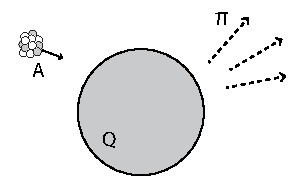
\includegraphics[scale=1.0]{qball-cartoon.pdf}
\caption{Interaction of a baryonic Q-ball with a nucleus $A$. The Q-ball destroys the nucleus and absorbs its baryonic charge, while the excess energy is radiated into roughly $A$ outgoing pions of energy $\Lambda_\text{QCD}$.}
\label{fig:qball-cartoon}
\end{figure}

\begin{figure}
\includegraphics[scale=.35]{Qballconstraint.pdf}
\caption{
Constraints on Q-ball DM.
Bounds come from demanding that the Q-ball interaction during a DM transit is capable of igniting WDs, occurring at a rate large enough to either ignite a single observed $1.25~M_{\astrosun}$ WD in its lifetime (WD in local DM density is blue shaded) or exceed the measured SN rate in our galaxy.
Also shown is the corresponding constraint from gravitational heating of WDs (orange shaded), and existing limits from terrestrial detectors (red)~\cite{Dine:2003ax}.}
\label{fig:Qballconstraint}
\end{figure}
